\documentclass[11pt,letterpaper]{article}

\usepackage[letterpaper,margin=0.8in,nohead]{geometry}

\usepackage[colorlinks]{hyperref}
\usepackage{url}
\usepackage{breakurl}

\hypersetup{
	colorlinks,
	linkcolor={red},
	citecolor={red},
	urlcolor={blue}
}

\usepackage{verbatim}
\usepackage{fancyvrb} 
\usepackage{scrextend}
\usepackage{enumitem}
\usepackage{url}
\usepackage{tabularx}

\usepackage{caption}
\usepackage{graphicx}
\usepackage{subcaption}

\usepackage{changepage}   % for the adjustwidth environment

\newenvironment{answer}{\em \color{blue} \begin{adjustwidth}{1cm}{1cm}}{\end{adjustwidth}}

% math
\usepackage{amsthm,amsmath}
\usepackage{amsfonts}

\newcommand{\mc}[1]{\mathcal{#1}}	% Mechanisms / Algorithms
\newcommand{\rv}[1]{\mathbf{#1}}    % Random variable

\newcommand{\pr}[1]{\mathrm{Pr}\{#1\}} % Probability

\newtheorem{corollary}{\bf Corollary}%[theorem]
\newtheorem{lemma}{\bf Lemma}%[theorem]
\newtheorem{definition}{\bf Definition}%[section]

\newtheorem{observation}{\bf Observation}%[theorem]

% load cleveref last!
\usepackage[capitalise]{cleveref}


\begin{document}
	
	\title{EN4720: Security in Cyber-Physical Systems \\ Exercise --- Authentication}
	
	%% This is an individual assignment!!
	%% TODO: put your name and index number here here!
	\author{ \textcolor{blue}{Name: Thalagala B. P.} \\ \textcolor{blue}{Index No: 180631J}}
	
	\maketitle
	
	\begin{center}
		\color{red}\bf This is an individual exercise! \\ Due Date: 19 May 2023 by 11.59 PM
	\end{center}
	
	\begin{center}
		\small Content adopted from the Udacity Security Engineer Nano-Degree and ECU CSI 1101.    
	\end{center}
	
	\vspace{1in}
	
	This exercise has to be carried out using a Linux-based PC/virtual machine. Read all the instructions and questions before attempting the exercise. Add answers under each question in the Questions section and submit the resulting PDF. All files used in this exercise can be found in {\it ex3-resources} folder.
	
	\subsection*{Instructions}
	
	\begin{enumerate}
		\item Explore and understand how Unix systems store and manage passwords.
		
		\item Download the shadow.hex file from the ``files'' folder. This file has been encrypted using RC4 encryption. 40 bits hexadecimal key: \textcolor{magenta}{5D 49 34 71 64}. Decrypt the file using any available decryption tool (e.g., cryptool).
		
		\item Download the ``500\_passwords.txt'' file from the “files” folder. Run ``hashcat'' password cracking utility to crack the passwords in the decrypted shadow file with the help of the dictionary ``500\_passwords.txt''. Please note that, to crack the passwords in the decrypted shadow file using hashcat, you need to take encrypted password fields of each user into a different file. You may rename that file as ``encrypted\_passwords.txt''.
		
		\item Download the ``myhashes.txt'', ``mydictionary.txt'', ``myruleset.txt''  files from the “files” folder. Note that, myhashes.txt containes MD5 hashes. Run a rule-based attack using “hashcat” password cracking utility to crack the passwords in the myhashes.txt file with the help of the dictionary “mydictionary.txt” and the ruleset myruleset.txt.
		
		\item Answer the questions given below.
		
	\end{enumerate}
	
	\newpage
	\subsection*{Questions}
	
	\begin{enumerate}
		
		\item What is the difference between \textcolor{magenta}{/etc/passwd} and \textcolor{magenta}{/etc/shadow} files? Complete Table~\ref{tab:difference-passwd-shadow}.
		
		\begin{answer}
			\textcolor{magenta}{/etc/passwd} file stores the account details of the users on a given host machine. The content of the file is word-readable and everyone has the read permission for that file. 
			
			\begin{verbatim}
			(user@host)-[/etc]
			$ ls -lh | grep passwd
			-rw-r--r--  1 root root   2.0K Apr  2 14:44 passwd
			-rw-r--r--  1 root root   2.0K Apr  2 14:38 passwd-
			\end{verbatim}
		
			\textcolor{magenta}{/etc/shadow} file stores the details about the passwords of users and hashed passwords. The shadow file can only be read by the root account.
			
			\begin{verbatim}
			(user@host)-[/etc]
			$ ls -lh | grep shadow
			-rw-r-----  1 root shadow  770 Apr  2 14:44 gshadow
			-rw-r-----  1 root shadow  761 Apr  2 14:44 gshadow-
			-rw-r-----  1 root shadow  968 Apr  2 14:44 shadow
			-rw-r-----  1 root shadow  949 Apr  2 14:38 shadow-
			\end{verbatim}
			
			\begin{table}[h!]
				\caption{Difference between /etc/passwd amd etc/shadow files} \label{tab:difference-passwd-shadow}
				\begin{tabularx}{\columnwidth}{|p{4cm}|X|X|}
					\hline
					\textbf{Attribute} & \textbf{/etc/passwd} & \textbf{etc/shadow} \\
					\hline
					Number of fields & 7 & 9\\\hline
					
					\hline
					Accessible users & Anyone can read& Only {\tt root} user and members of {\tt shadow} group can read \\\hline
				\end{tabularx}
			\end{table}
			
		\end{answer}
		
		
		
		\item You will find seven fields in the /etc/passwd file as indicated in Figure~\ref{fig:etc-passwd-format}. Explain the purpose of each field.
		
		\begin{figure}[h]
			\centering
			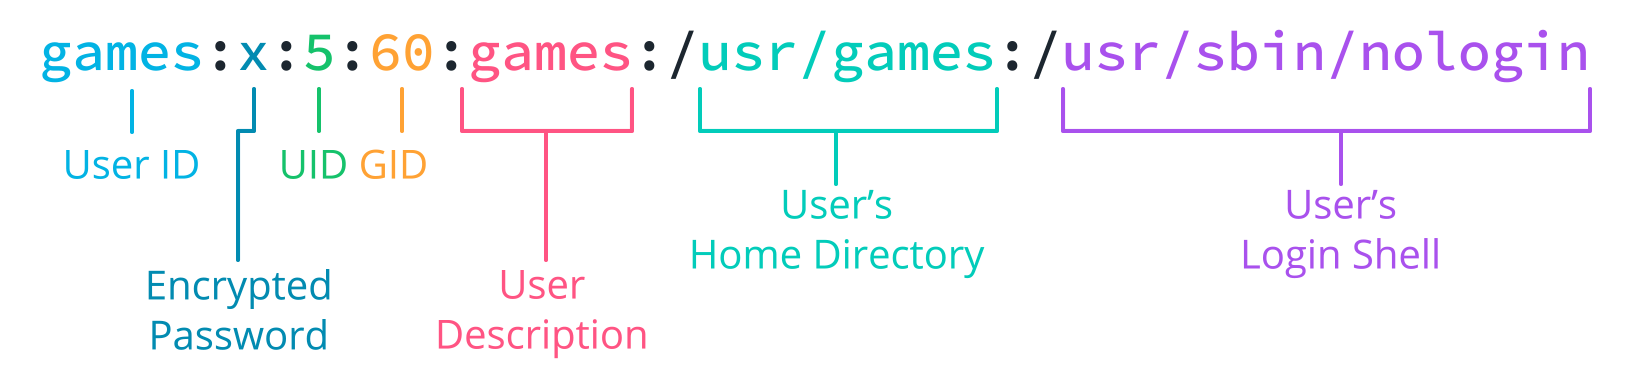
\includegraphics[width=0.7\columnwidth]{images/ex3-etc-passwd-format.png}
			\caption{Example storage format of /etc/passwd file} \label{fig:etc-passwd-format}
		\end{figure}
		
		\begin{answer}
			\begin{enumerate}
				\item {\tt games}: name of the user for whom this entry corresponds to.
				\item {\tt x} : indicates that a password exists for the user. However, the password is stored in the \textcolor{magenta}{/etc/shadow} file. If instead of x it shows a ! symbol, this indicates that a password does not exist.
				\item {\tt 5} : User ID of this user. User IDs for created users begin from 1000 and run up to 59999
				\item {\tt 60}: Group ID of the group this user belongs to.
				\item {\tt games}: can contain multiple comma separated sub-fields of information inclusive of full name and telephone numbers. Here, no telephone numbers have been provided.
				\item {\tt /usr/games} : location of home directory assigned to this user.
				\item {\tt /usr/sbin/nologin} : default shell assigned to this user.
			\end{enumerate}
			
			
			
		\end{answer}
		\textbf{Note}: Information adopted from,  \\\url{https://www.maketecheasier.com/how-linux-stores-manages-user-passwords/}
		
		
		
		\item Dump the content of your /etc/shadow file to the terminal using \textcolor{magenta}{sudo cat /etc/shadow} and add a screenshot.
		
		\begin{answer}
		\begin{figure}[h]
			\centering
			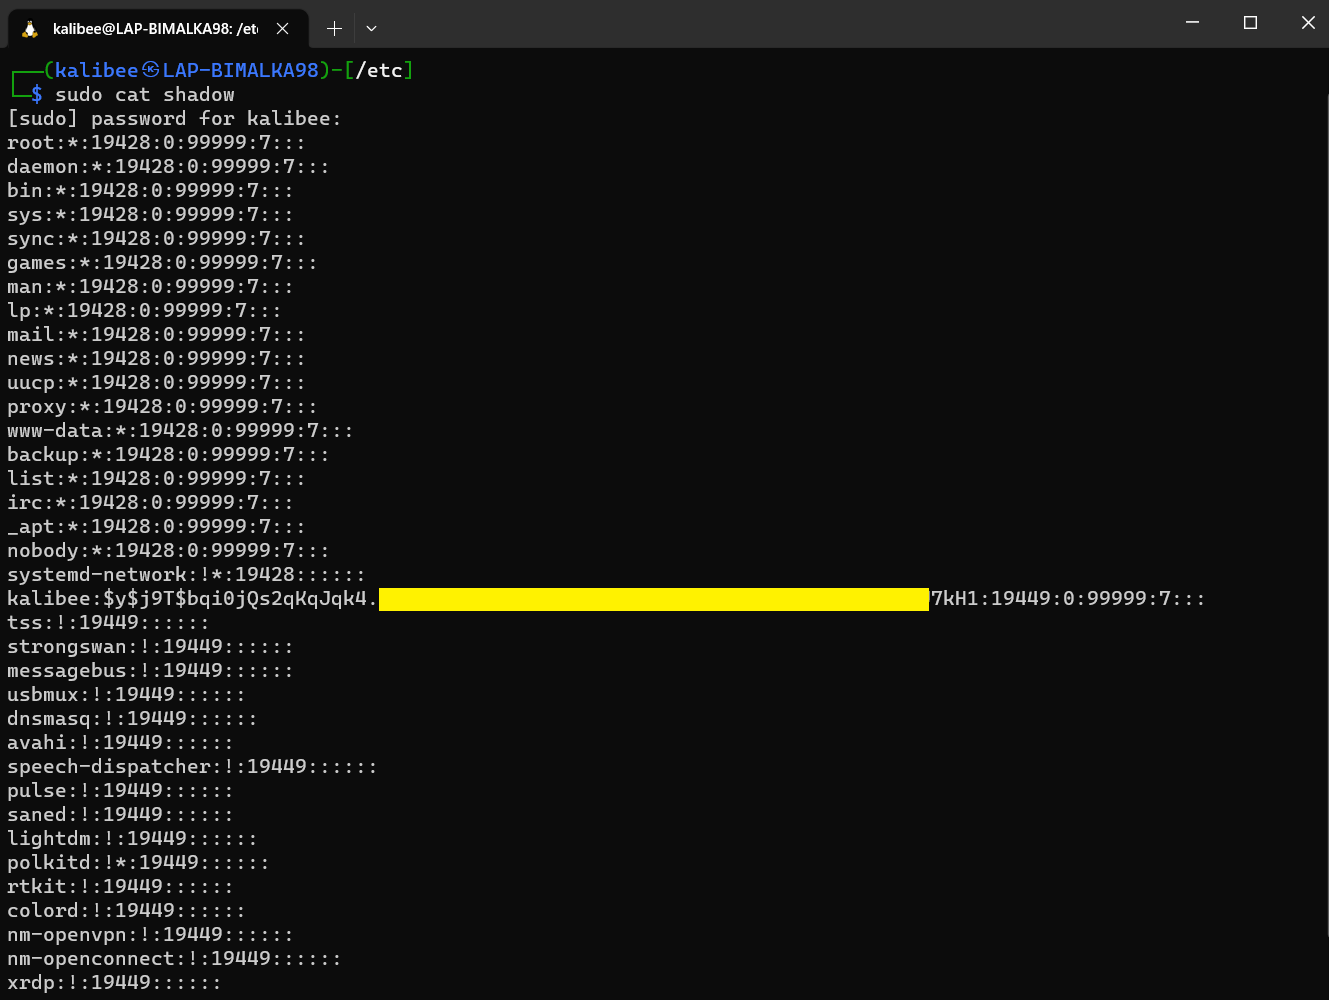
\includegraphics[width=0.8\columnwidth]{images/myshadow}
			\caption{Content of /etc/shadow file} \label{fig:myshadow}
		\end{figure}
		\end{answer}
		
		\item Identify the different fields present in one line in the shadow file and explain the purpose of each field. Clearly mark the fields and provide the explanation.
		
		\begin{answer}
			there are 9 fields in an entry in the shadow file, and each field can be identified as follows. Let us consider the entry of the user ``kalibee''
			
			\begin{enumerate}
				\item {\tt kalibee} - name of the user for whom this entry corresponds to
				\item {\tt \$y\$j9T\$bqi0jQs2qKqJqk4...7kH1} - hashed user password. Along with the information about, the hashing algorithm, used salt value.
				\item {\tt 19449} - last password change time (in days since Jan 1, 1970)
				\item {\tt 0} - the number of days after which the password can be changed. A value of 0 means the password can be changed at any time.
				\item {\tt 99999} - the number of days after which the password must be changed. A value of 99999 indicates a user can retain the password as long as desired.
				\item {\tt 7} -  if the password is set to expire, this fields indicates the number of days to warn the user about password expiry.
				\item {\tt :::} - Three empty fields. The first one indicates the number of days to wait after password expiry, following which the account will be disabled. The second one indicates the number of days since January 1, 1970, that an account has been disabled. The third field is reserved for future use. The empty fields indicate that the existing password for this user has not expired and is not set to expire soon.
			\end{enumerate}
		\end{answer}
		
		\textbf{Note}: Information adopted from,  \\\url{https://www.maketecheasier.com/how-linux-stores-manages-user-passwords/}
		
		\item Complete Step \#2 mentioned under \textbf{Instructions}. Add a screenshot of the decrypted shadow.hex file content. What is the type of hash in the decrypted shadow file?
		
		\begin{answer}
			\begin{figure}[h]
				\centering
				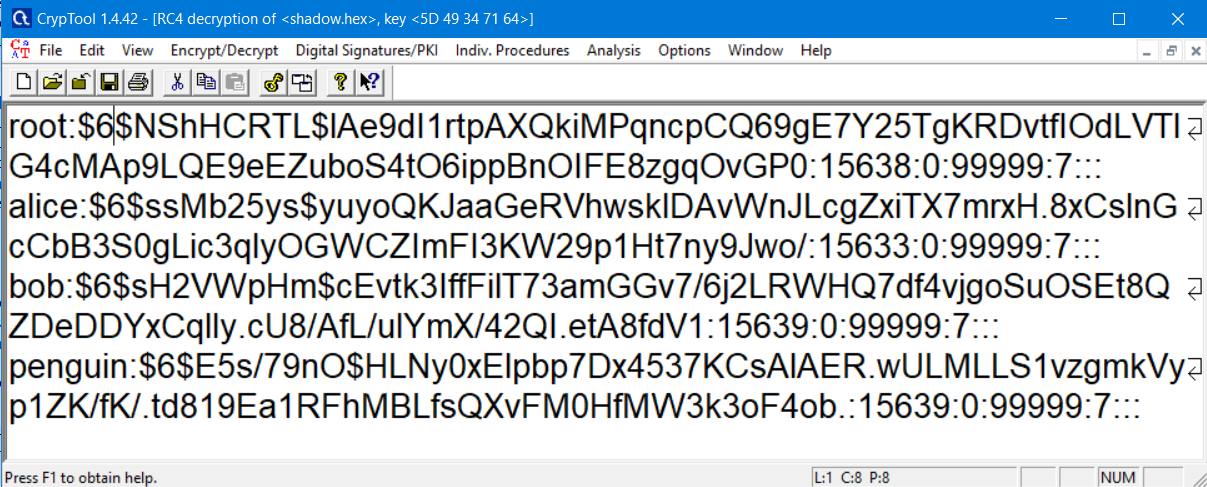
\includegraphics[width=0.7\columnwidth]{images/shdwdecrypt}
				\caption{Content of the decrypted shadow.hex file using the key \textcolor{magenta}{5D 49 34 71 64}} \label{fig:shadow.hex}
			\end{figure}
		
		All the password hashes start with hash ID, \$6\$. This indicates that they use SHA-512 hashing algorithm.
		
		\end{answer}
		
		\item Complete Step \#3 mentioned under \textbf{Instructions}. Add a screenshot of a part of the ``500\_passwords.txt'' file content using vi/vim/nano.
		
		\begin{answer}
			\begin{figure}[h]
				\centering
				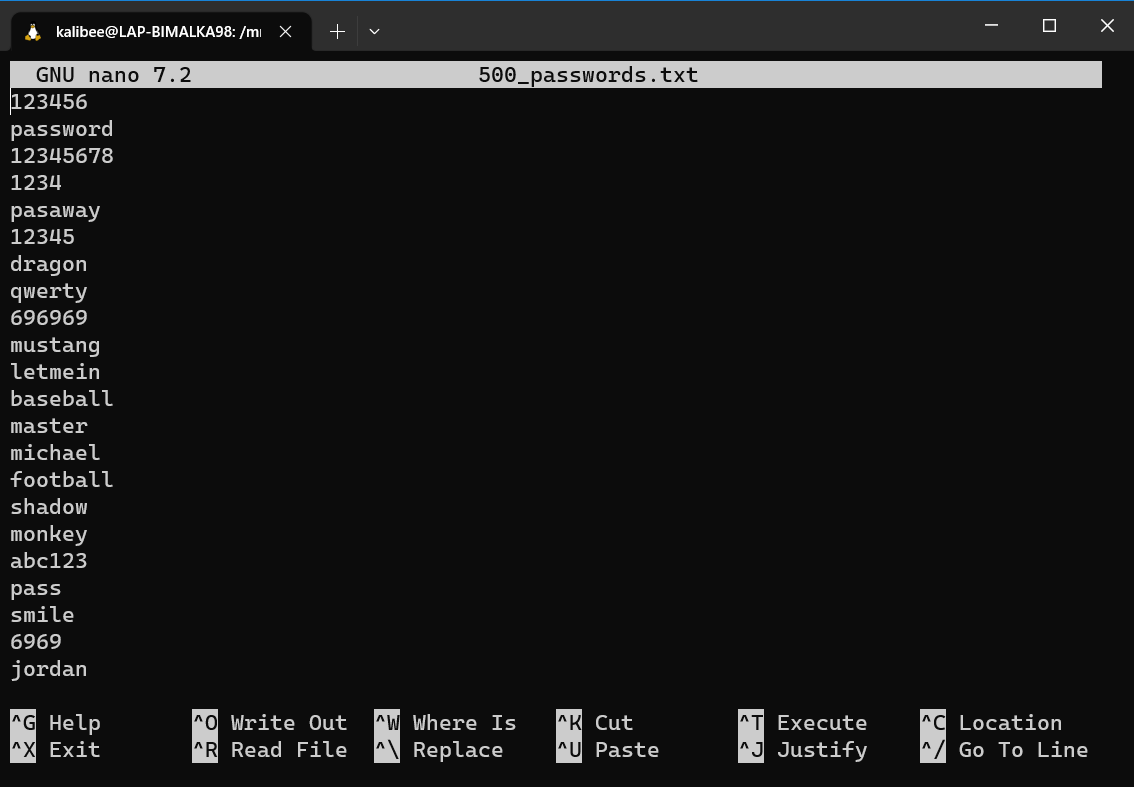
\includegraphics[width=0.7\columnwidth]{images/dict_500}
				\caption{A part of the content of ``500\_passwords.txt'' file} \label{fig:dict_500}
			\end{figure}
		\end{answer}
		
		\item What is the command you used to crack the passwords in the shadow file? Briefly explain each field in the command.
		
		\begin{answer}
			
			\begin{verbatim}
				hashcat -m 1800 -a 0 encrypted_passwords.txt 500_passwords.txt
				    --potfile-path=cracked.pot
			\end{verbatim}
			
			\begin{itemize}
				\item {\tt -m 1800} specifies the code for the hash mode: 1800 -  sha512crypt \$6\$, SHA512 (Unix) in the category of `Operating System'.
				
				\item {\tt -a 0} specifies the `Straight' attack mode that is dictionary attack.
				
				\item An optional parameter can be passed to specify the path to the `.pot' file, where the cracked passwords are saved. {\tt --potfile-path=cracked.pot}. This will save the pot file in the same directory as the other input files.
			\end{itemize}
			
			
		\end{answer}
		
		\item Add a screenshot of all the cracked passwords.
		
		\begin{answer}
			\begin{figure}[h]
				\centering
				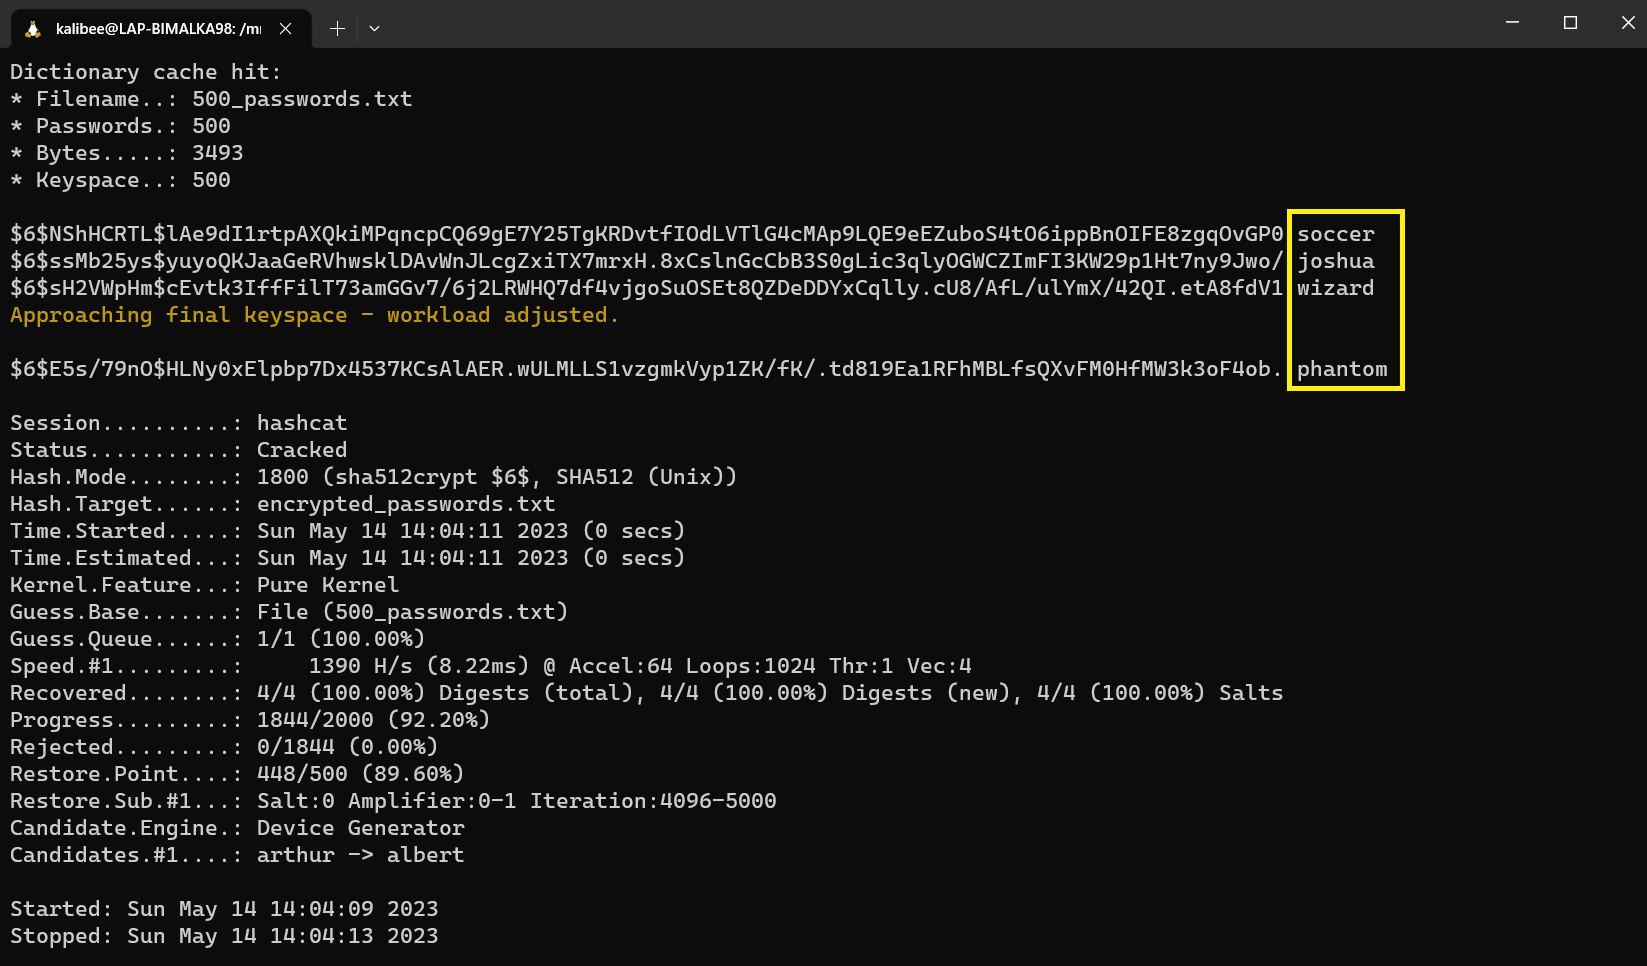
\includegraphics[width=0.9\columnwidth]{images/cracked_shadow}
				\caption{Cracked passwords using Hashcat tool} \label{fig:cracked_shadow}
			\end{figure}
		\end{answer}
		
		\item Provide recommendations to enhance the strength of the passwords.
		
		\begin{answer}
		\begin{itemize}
			\item When creating a password a combination of numbers, letters (upper case and/or lower case)  and special characters must be used and the password must be sufficiently long to make it stronger.				
			
			\item When creating a password common words (such as \textit{soccer, wizard, phantom (found above)  and etc} ) and patterns (such as \textit{123, 12345 and etc} ) must be strictly avoided. As these words can be easily cracked in no time as seen in the above scenario.					
			
			\item A password must not contain personal information such as name, birth year and etc. as those can easily be combined to form a candidate set of passwords easily.
		\end{itemize}
		\end{answer}
		
		\item Briefly explain about ``Rule-based Attack'' and how it uses time and memory for the hash cracking process using a diagram.
		
		\begin{answer}
			While pure dictionary attacks use the bare passwords in a given file, rule-based attacks can generate new candidate passwords using a dictionary of passwords. In order to to do that, password cracking tools have functions to modify, cut or extend words and has conditional operators to skip some, etc. That makes it the most flexible, accurate and efficient attack. Due to the complexity of the process it uses more time and more memory for the attack.
		\end{answer}
	
		\textbf{Note}: Information adopted from,  \\\url{https://hashcat.net/wiki/doku.php?id=rule_based_attack}
		
		\item Complete Step \#4 mentioned under \textbf{Instructions}. Add a screenshot of the mydictionary.txt and myruleset.txt file contents. Define each rule in myrulset.txt using standard rules in the rule-based attack.
		
		\begin{answer}
			\begin{figure}[h]
				\centering
				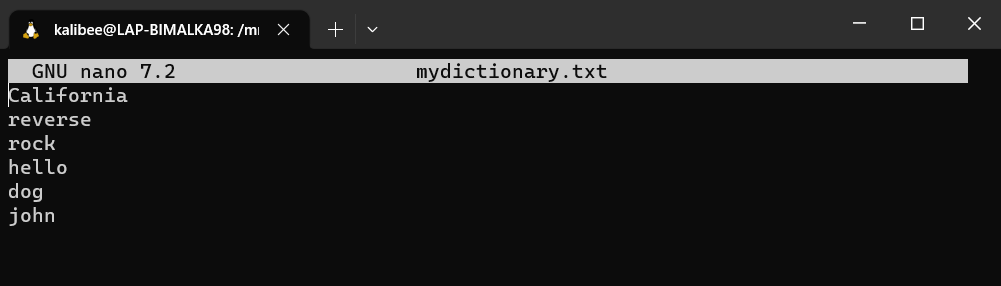
\includegraphics[width=0.7\columnwidth]{images/mydict}
				\caption{Content of the {\tt mydictionary.txt} file} \label{fig:mydict}
			\end{figure}
		
			\begin{figure}[h]
				\centering
				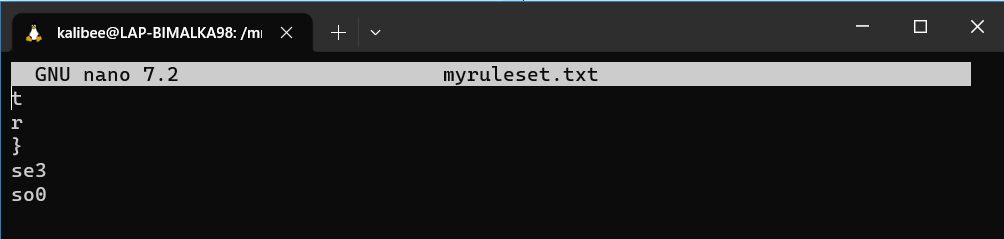
\includegraphics[width=0.7\columnwidth]{images/myrules}
				\caption{Content of the {\tt myruleset.txt} file} \label{fig:myrules}
			\end{figure}
		
		Definitions of the rules shown in the Figure \ref{fig:myrules},
		
		\begin{itemize}
			\item {\tt t} - Toggle the case of all characters in word.
			\item {\tt r} - Reverse the entire word
			\item {\tt \}} - Rotate the word right
			\item {\tt se3} and {\tt so0}- (sXY) Replace all instances of X with Y
		\end{itemize}
		
		\end{answer}
		
		\item Add a screenshot of all the cracked passwords. Run a dictionary attack without myruleset.txt (using only the dictionary) and compare the two cracked files.
		
		\begin{answer}
			
			Through the rule-based attack, the tool can generate new candidate passwords other than the original password set. This increases the keyspace to 30 passwords from only 6 passwords, which increases the effectiveness of the attack. Figure \ref{fig:cracked_with_rules} illustrates that, through the rule-based attack, all the six passwords are cracked, whereas  only one password is cracked through the bare dictionary attack (figure \ref{fig:cracked_with_norules}) .
			
			\begin{figure}[h]
				\centering
				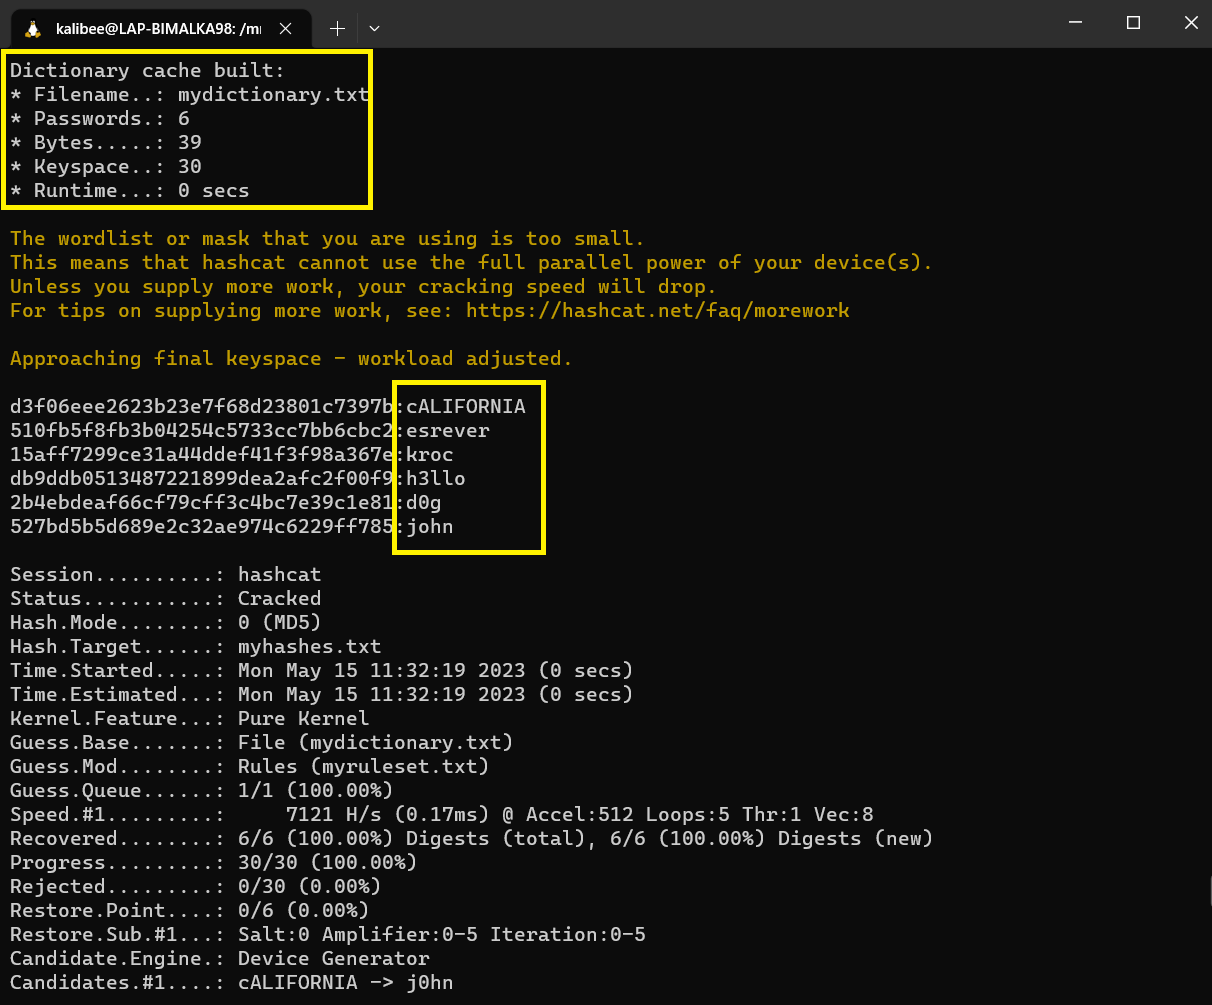
\includegraphics[width=0.7\columnwidth]{images/cracked_with_rules}
				\caption{Cracked passwords using the rule-based attack. \textbf{Command} : {\tt hashcat -m 0 -a 0 myhashes.txt mydictionary.txt -r myruleset.txt --potfile-path=cracked.pot}} \label{fig:cracked_with_rules}
			\end{figure}
			
			\begin{figure}[h]
				\centering
				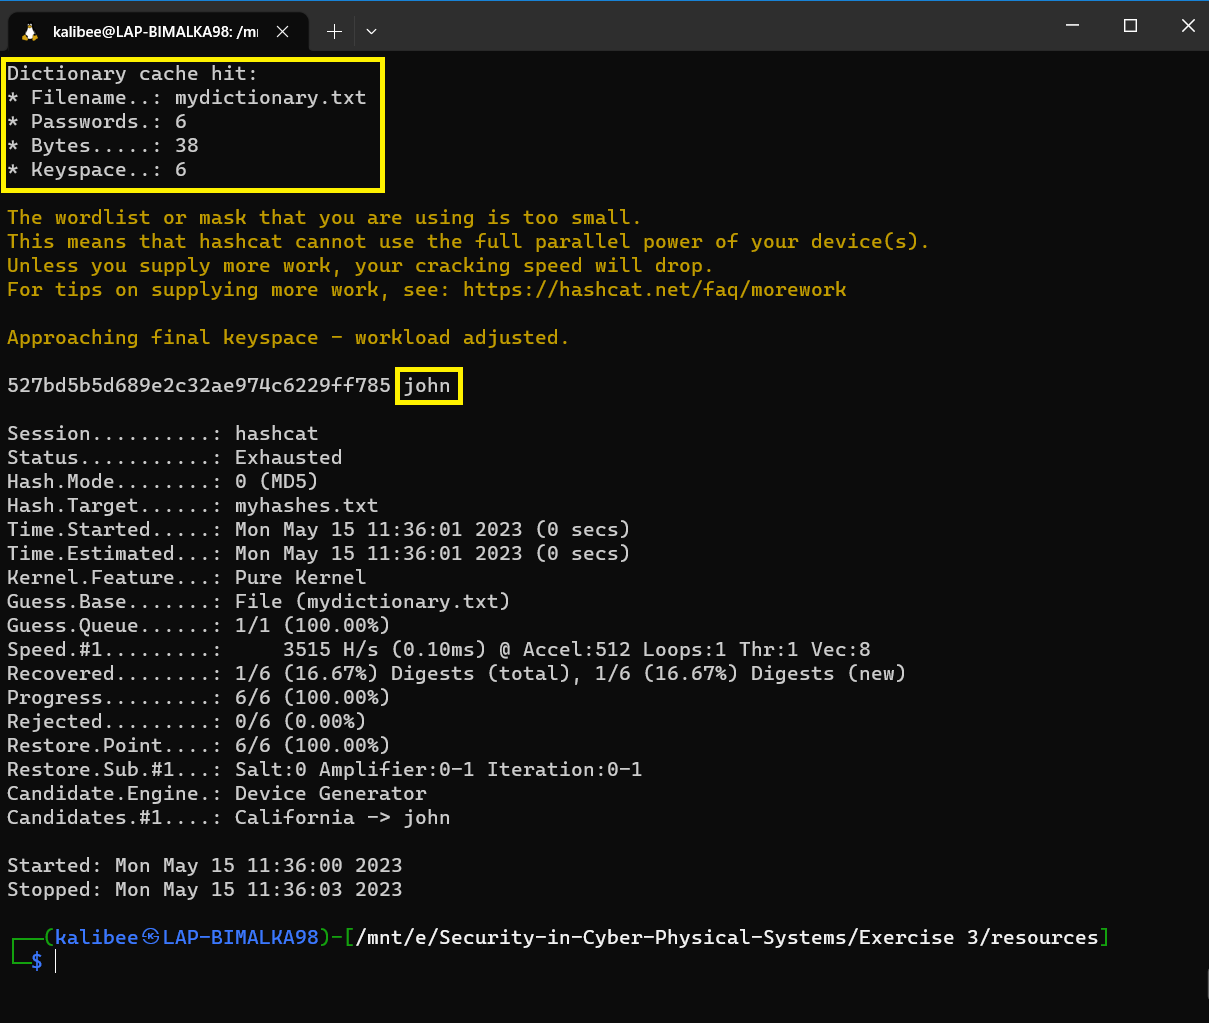
\includegraphics[width=0.7\columnwidth]{images/cracked_with_norules}
				\caption{Cracked passwords using bare dictionary attack. \textbf{Command} : {\tt hashcat -m 0 -a 0 myhashes.txt mydictionary.txt --potfile-path=cracked.pot}} \label{fig:cracked_with_norules}
			\end{figure}
		\end{answer}
		
	\end{enumerate}
	
\end{document}